\maketitle
\tableofcontents
\newpage

\begin{otherlanguage}{russian}
  \begin{abstract}
    Пусть есть прибор, который в дискретные моменты времени выдаёт сигнал по закону $f(t) = sin \pi t$. Допустим, наблюдатель зарегистрировал пятьотсчётов в моменты времени $t_{i} = \frac{i}{4}, i = 0, 1, 2, 3, 4$. Задачей наблюдателя(который не знает закона выдачи сигнала) является получение приближённого значения функции на отрезке $[0, 1]$ в любой момент времени.
  \end{abstract}
\end{otherlanguage}

\section{Первое задание}

Используя линейную интерполяцию, найдите значения функции в точках: $t = 0, \frac{1}{6}, \frac{1}{3}, \frac{1}{2}$ и сравните с реальным значением синуса в этих точках. Постройте графики синуса и ломаной, проходящей через пять заданных точек. Отметьте, насколько сильно они различаются в разных частяхграфика. Чем это обусловлено?\\[5mm]

Формула линейной интерполяции:
\[
  f(x) = f(x_{i}) + \frac{f(x_{i+1}) - f(x_{i})}{x_{i+1} - x_{i}}(x - x_{i})
\]

\lstinputlisting{code/first_task.m}
\begin{lstlisting}[backgroundcolor=\color{lime}]
  y =

        0        0
   0.4714   0.5000
   0.8047   0.8660
   1.0000   1.0000
 \end{lstlisting}

\begin{figure}[h]
  \centering
  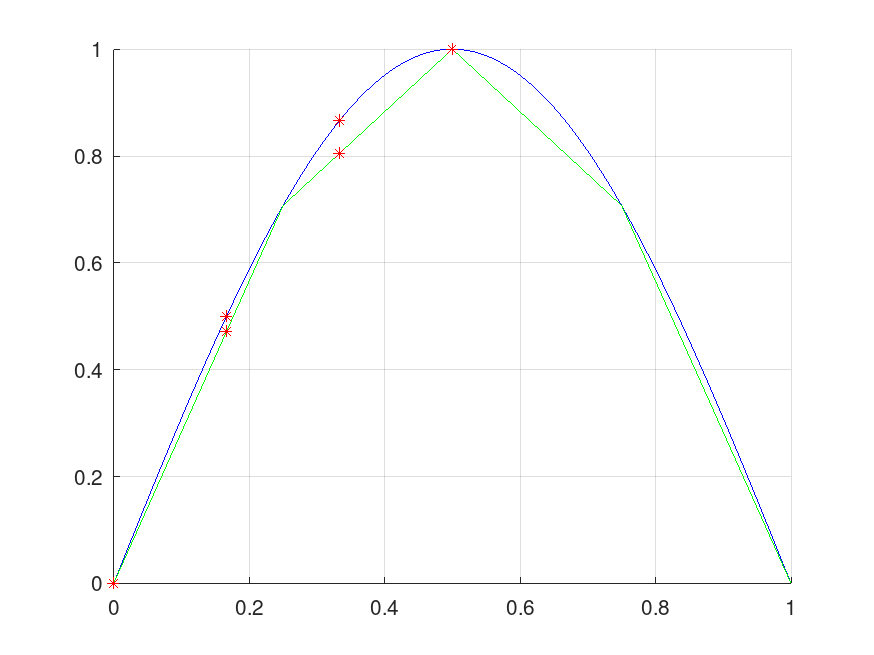
\includegraphics[width=0.8\textwidth]{images/first_task_1.png}
\end{figure}

\section{Второе задание}
